\subsection{Runtime Calibration} \label{sec:calibration}
During RAT, we differentiate between known and unknown rts's. 
Known rts's are those which have been encountered during DTA. So the optimal configuration for the rts's is known. 
However, unknown rts's describe those which have not been encountered during DTA. 
There are several reasons why unseen rts's might occur. 
First, an unseen rts may consists of already known regions, but with unknown user parameters that were not present during DTA or parameters that might have changed between DTA and runtime. Typically, these changes are related to different application inputs. 
Second, an unseen rts may consist of completely new regions, which were not seen during DTA. 
The goal of the calibration is to handle these unknown rts's during RAT.

Since, the calibration is done during the production run, there are a few restrictions which had to be taken in account for the design of calibration mechanism. 
First, there can be no user input and 
second, a good configuration has to be found in short time. 
A DTA like approach for searching optimal configuration is not feasible as it would degrade the performance of the application.

For runtime calibration, we provide two different Machine Learning based approaches. The first approach is a Q-Learning based mechanism. The algorithm starts at the maximal core and uncore frequency. With a probability of {$\epsilon$}, the algorithm selects a different setting from the next direct neighbours. Then it measures the energy at this point. Based on that, it calculates a so-called Q-Value. Afterwards, the algorithm chooses the next optimal status according to the Q-Value and starts from the beginning. Figure~\ref{fig:qlearning} shows how the mechanism searches for an energy efficient optimum (core frequency = 2.3 GHz, uncore frequency = 2.2 GHz) starting from a selected initial setting (core frequency = 1.9 GHz, uncore frequency = 2.2 GHz).
\begin{figure}[!t]
\centering
%\includegraphics[trim={7cm 2cm 5.5cm 2cm},clip,width=3in]{readex-approach}
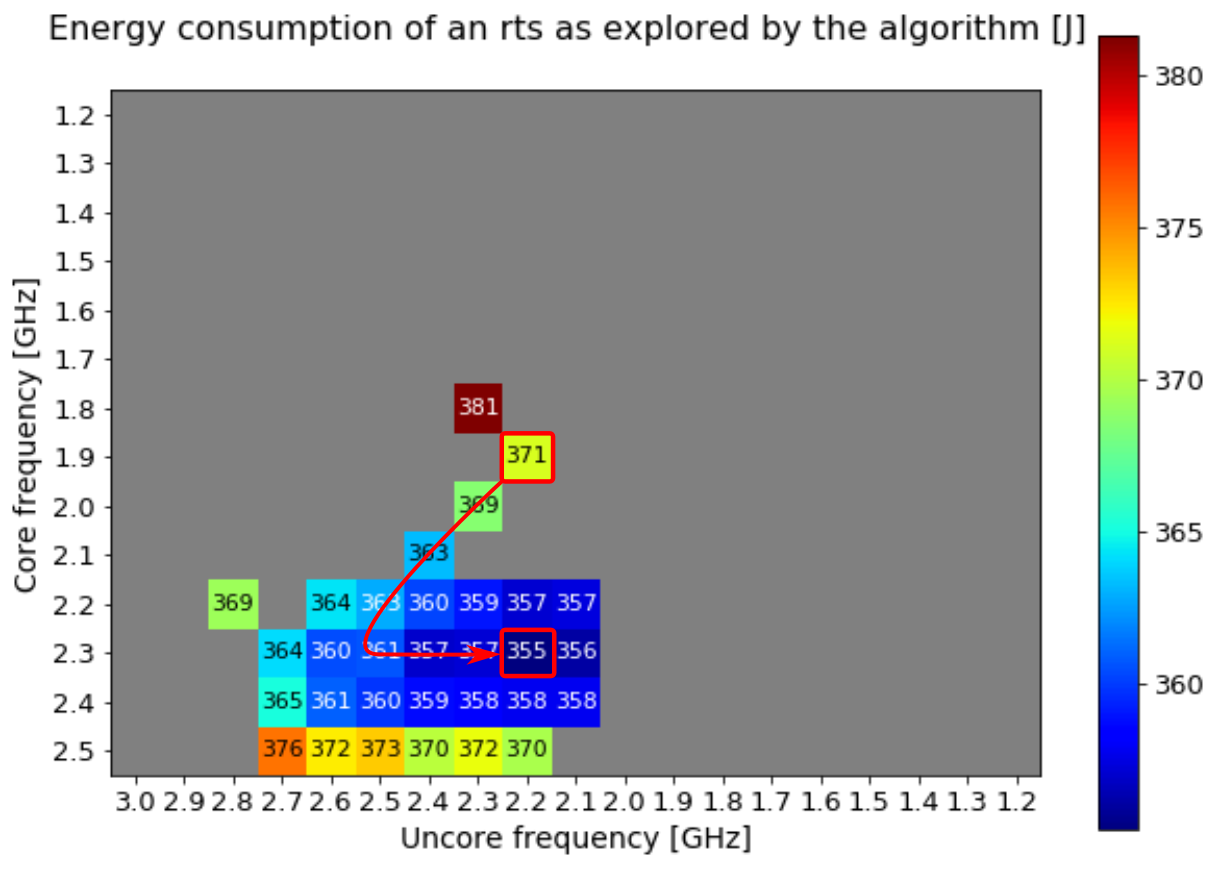
\includegraphics[width=.8\columnwidth]{figures/q_learning.png}
\caption{Heatmap of energy consumption of a specific region for different core and uncore frequencies as explored by a Q-Learning algorithm applied at runtime. The algorithm starts at 1.9/2.2 GHz and finds a more suitable setting (2.3/2.2 GHz).}
\label{fig:qlearning}
\end{figure}
In the second approach, we used performance counters to predict the optimal setting using Neural Networks. First, the approach identifies the most relevant performance counters. In a second step, it trains a shallow neural network in order to predict a good frequency. This model is then loaded during runtime. Once the RRL encounters an unseen RTS, it measures the relevant performance counters and uses the neural network to predict a good setting. In opposite to the Q-Learning approach, this approach does require a pre-training, which has to be performed once per system. However, once this is done, the network just needs to be evaluated, which requires less tuning and runtime overhead compared to the Q-Learning approach. 


